\section{Laboratory work implementation}

\subsection{Tasks and Points}

\begin{itemize}
	\item Realizeaza un simplu GUI calculator care suporta urmatoare functii: +, -, /, *, putere, radical. 
	\item InversareSemn(+/-), operatii cu numere zecimale.
	\item Divizare proiectului in doua module - Interfata grafica(Modul GUI) si Modulul de baza(Core Module).
\end{itemize}

\subsection{Analiza lucrarii de laborator}

Repository \url{https://github.com/dragosh1011/MIDPS-laboratories/tree/master/MIDPS/LAB_2}{link}

Pentru ralizarea acestei aplicatii am utilizat visual studio ide si c sharp. 
Crearea unui calculator utilizand c sharp este o sarcina destul de simpla. Partea logica a aplicatiei este destul de simpla si consta din cateva metode simple care fac operatiile necesare intre 2 numere sau 1, daca e vorba de radical sau inversare semn. Aceste metode se afla in modulul core al aplicatiei si reprezinta un singur fisier calculator.cs care contine 7 operatii. Pentru a realiza operatiile de ridicare la putere sau radical se utilizeaza modulul Math care ofera mai multe metode din matematica. 
Modulul de grafica se afla in GUI si consta dintr-o forma ce contine 22 de butoane, 1 textBox si un label. Aici se afla si metodele de parsare a textului introdus si se determina operatiile care sunt solicitate. Dupa determinarea numerelor si a operatiei necesare de efectuat din acest modul se apeleaa metodele din modulul Core pentru a obtine reultatul.

Problemele intilnite la acest laborator tin in mare parte de deprinderile acumulate in utilizarea limbajului javascript, care este un limbaj netipizat fata de C Sharp. 

\break
\subsection{Imagini}

\begin{center}
	\begin{figure}[h]
		\centering
		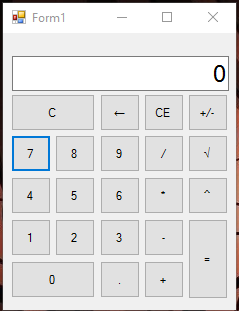
\includegraphics[width=10cm]{calculator}\\
		\caption{Calculator}
		\label{run}
	\end{figure}
	
	\begin{figure}[h]
		\centering
		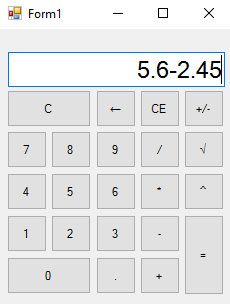
\includegraphics[width=10cm]{zecimale}\\
		\caption{Operations}
		\label{jump}
	\end{figure}
	
	\begin{figure}[h]
		\centering
		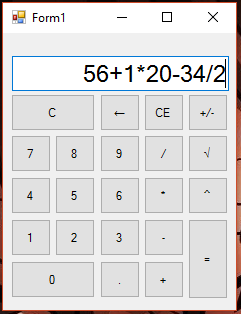
\includegraphics[width=10cm]{multiple-operations}\\
		\caption{Multiple operations}
		\label{slide}
	\end{figure}
\end{center}

\clearpage